\documentclass[letterpaper,12pt,fleqn]{article}
\usepackage{matharticle}
\usetikzlibrary{decorations.markings}
\pagestyle{empty}
\renewcommand{\o}{\theta}
\begin{document}
\section*{Mappings}

\begin{itemize}
\item A function $f$ is a \emph{mapping} from the $z$-plane to the $w$-plane,
  such that the coordinates $(x,y)$ are mapped to coordinates $(u,v)$.

  \begin{tikzpicture}
    \draw [<->] (-1,0) -- (4,0);
    \draw [<->] (0,-1) -- (0,4);
    \node [right] at (4,0) {$x$};
    \node [above] at (0,4) {$y$};
    \draw [fill=gray!30,rounded corners=0.1in] (2,2) \blob{0.6in}{0.1in};
    \node at (2,1) {$D$};
    \draw [fill=black] (2,2) circle [radius=0.05];
    \node [below left] at (2,2) {$z$};

    \draw [<->] (6,0) -- (11,0);
    \draw [<->] (7,-1) -- (7,4);
    \node [right] at (11,0) {$u$};
    \node [above] at (7,4) {$v$};
    \draw [fill=gray!30,rounded corners=0.1in] (9,2) \blob{0.6in}{0.1in};
    \node at (9,1) {$R$};
    \draw [fill=black] (9,2) circle [radius=0.05];
    \node [below right] at (9,2) {$w$};

    \draw [dashed] (2,2) to [out=45,in=135] (8.9,2.1);
    \node at (5,4) {$f(z)$};
\end{tikzpicture}

\item The region $D$ is called the \emph{domain} and the region $R$ is called
  the range.

\item The value $w$ is called the \emph{image} of $z$ under $f$, and the value
  $z$ is called the \emph{pre-image} of $w$.

\item Functions can be \emph{multi-valued}; there can be more than one
  pre-image for every image.
\end{itemize}

\begin{example}
  Translation of the Unit Square

  $f(z)=z+2$

  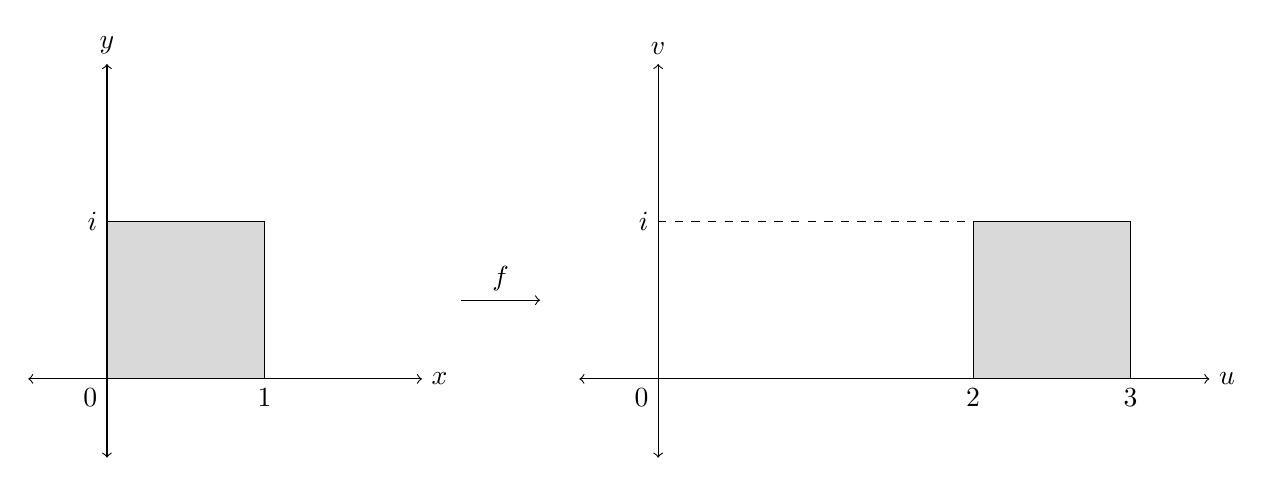
\begin{tikzpicture}
    \draw [<->] (-1,0) -- (4,0);
    \draw [<->] (0,-1) -- (0,4);
    \node [right] at (4,0) {$x$};
    \node [above] at (0,4) {$y$};
    \draw [fill=gray!30] (0,0) rectangle (2,2);
    \node [below left] at (0,0) {$0$};
    \node [below] at (2,0) {$1$};
    \node [left] at (0,2) {$i$};

    \draw [<->] (6,0) -- (14,0);
    \draw [<->] (7,-1) -- (7,4);
    \node [right] at (14,0) {$u$};
    \node [above] at (7,4) {$v$};
    \draw [fill=gray!30] (11,0) rectangle (13,2);
    \node [below left] at (7,0) {$0$};
    \node [below] at (11,0) {$2$};
    \node [below] at (13,0) {$3$};
    \node [left] at (7,2) {$i$};
    \draw [dashed] (7,2) -- (11,2);

    \draw [->] (4.5,1) -- (5.5,1);
    \node [above] at (5,1) {$f$};
  \end{tikzpicture}
\end{example}

\begin{example}
  Rotation by $90^{\circ}$

  $f(z)=iz$

  $f(z)=ire^{i\o}=e^{i\frac{\pi}{2}}re^{i\o}=re^{i(\o+\frac{\pi}{2})}$

  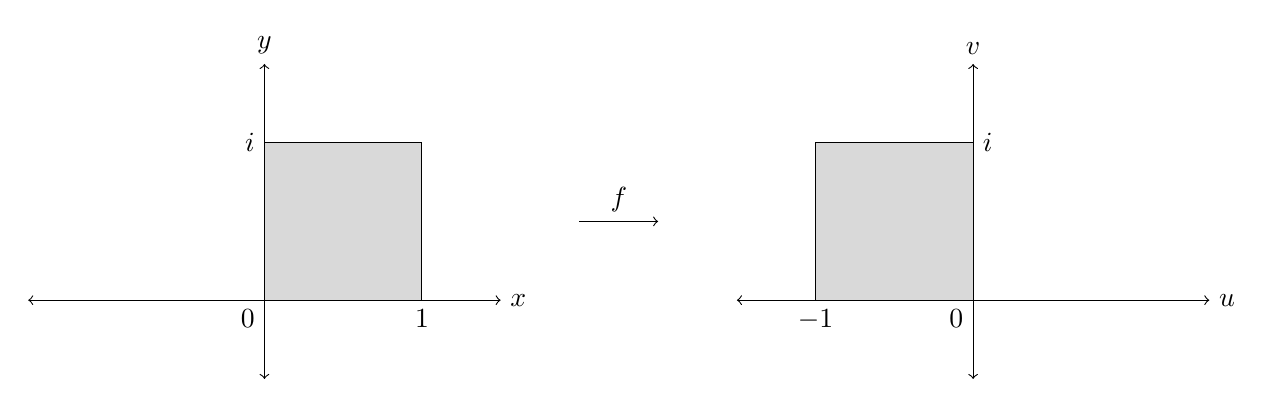
\begin{tikzpicture}
    \draw [<->] (-3,0) -- (3,0);
    \draw [<->] (0,-1) -- (0,3);
    \node [right] at (3,0) {$x$};
    \node [above] at (0,3) {$y$};
    \draw [fill=gray!30] (0,0) rectangle (2,2);
    \node [below left] at (0,0) {$0$};
    \node [below] at (2,0) {$1$};
    \node [left] at (0,2) {$i$};

    \draw [<->] (6,0) -- (12,0);
    \draw [<->] (9,-1) -- (9,3);
    \node [right] at (12,0) {$u$};
    \node [above] at (9,3) {$v$};
    \draw [fill=gray!30] (7,0) rectangle (9,2);
    \node [below left] at (9,0) {$0$};
    \node [below] at (7,0) {$-1$};
    \node [right] at (9,2) {$i$};

    \draw [->] (4,1) -- (5,1);
    \node [above] at (4.5,1) {$f$};
  \end{tikzpicture}
\end{example}

\begin{example}
  $f(z)=(1+z)^2$ on the unit disk

  Consider the boundary:
  \begin{eqnarray*}
    z &=& e^{i\o} \\
    w &=& (1+e^{i\o})^2 \\
    &=& (1+\cos\o+i\sin\o)^2 \\
    &=& \left(2\cos^2{\frac{\o}{2}}+
    i2\sin{\frac{\o}{2}}\cos{\frac{\o}{2}}\right)^2 \\
    &=& \left(2\cos{\frac{\o}{2}}\right)^2\left(\cos{\frac{\o}{2}}+
    i\sin{\frac{\o}{2}}\right)^2 \\
    &=& \left(4\cos^2{\frac{\o}{2}}\right)\left(e^{i\frac{\o}{2}}\right)^2 \\
    &=& 2(1+\cos\o)e^{i\o} \\
  \end{eqnarray*}
  $\rho=2(1+\cos\o)$\hspace{0.25in}$\phi=\o$

  \begin{minipage}[t]{3.5in}
    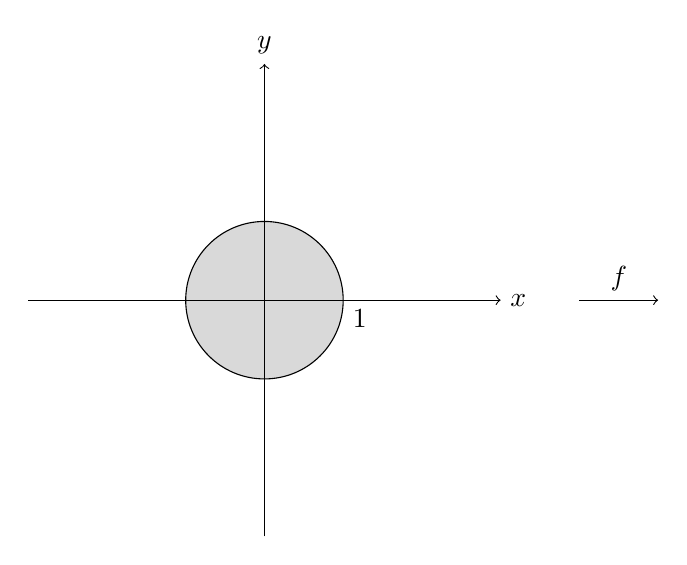
\begin{tikzpicture}
      \draw [fill=gray!30] (0,0) circle [radius=1];
      \draw [->] (-3,0) -- (3,0);
      \draw [->] (0,-3) -- (0,3);
      \node [right] at (3,0) {$x$};
      \node [above] at (0,3) {$y$};
      \node [below right] at (1,0) {$1$};

      \draw [->] (4,0) -- (5,0);
      \node [above] at (4.5,0) {$f$};
    \end{tikzpicture}
  \end{minipage}
  \begin{minipage}[t]{3in}
    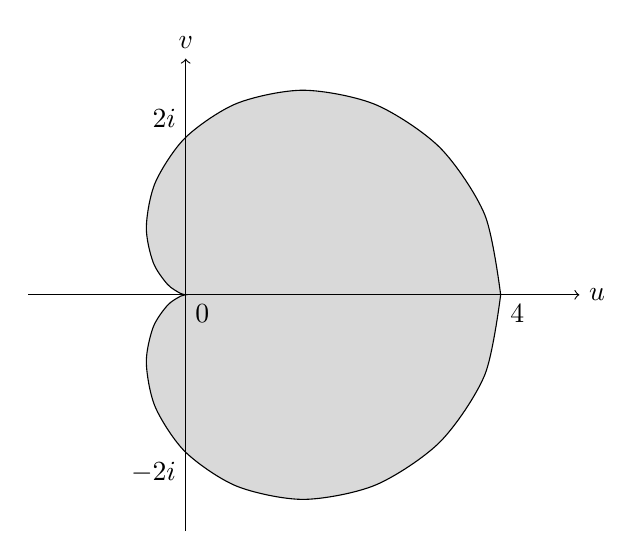
\begin{tikzpicture}
      \draw [fill=gray!30,domain=0:360,smooth] plot(xy polar cs:angle=\x,
      radius={2+2*cos(\x)});
      \draw [->] (-2,0) -- (5,0);
      \draw [->] (0,-3) -- (0,3);
      \node [right] at (5,0) {$u$};
      \node [above] at (0,3) {$v$};
      \node [below right] at (0,0) {$0$};
      \node [below right] at (4,0) {$4$};
      \node [above left] at (0,2) {$2i$};
      \node [below left] at (0,-2) {$-2i$};
    \end{tikzpicture}
  \end{minipage}
\end{example}
\newpage
\begin{example}
  $f(z)=e^z$ on a rectangular region

  $w=e^z=e^{x+iy}=e^xe^{iy}$

  $\rho=e^x$\hspace{0.25in}$\phi=y$

  \bigskip

  \begin{minipage}[t]{3in}
    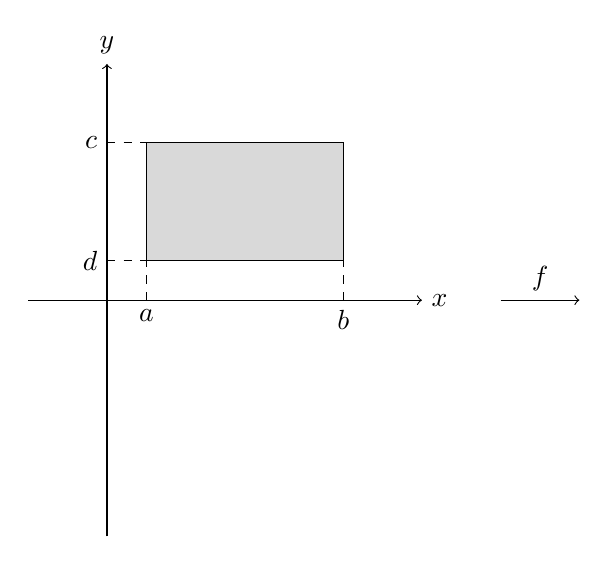
\begin{tikzpicture}
      \draw [->] (-1,0) -- (4,0);
      \draw [->] (0,-3) -- (0,3);
      \node [right] at (4,0) {$x$};
      \node [above] at (0,3) {$y$};
      \draw [fill=gray!30] (0.5,0.5) rectangle (3,2);
      \draw [dashed] (0.5,0) -- (0.5,0.5);
      \draw [dashed] (0,0.5) -- (0.5,0.5);
      \draw [dashed] (0,2) -- (1,2);
      \draw [dashed] (3,0) -- (3,0.5);
      \node [below] at (0.5,0) {$a$};
      \node [below] at (3,0) {$b$};
      \node [left] at (0,2) {$c$};
      \node [left] at (0,0.5) {$d$};

      \draw [->] (5,0) -- (6,0);
      \node [above] at (5.5,0) {$f$};
    \end{tikzpicture}
  \end{minipage}
  \begin{minipage}[t]{3in}
    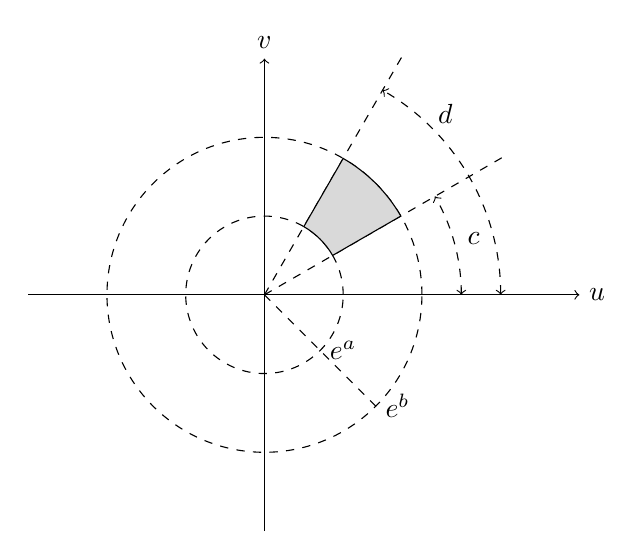
\begin{tikzpicture}
      \draw [->] (-3,0) -- (4,0);
      \draw [->] (0,-3) -- (0,3);
      \node [right] at (4,0) {$u$};
      \node [above] at (0,3) {$v$};
      \draw [dashed] (0,0) circle [radius=1];
      \draw [dashed] (0,0) circle [radius=2];
      \draw [dashed] (0,0) -- ({3.5*cos(60)},{3.5*sin(60)});
      \draw [dashed] (0,0) -- ({3.5*cos(30)},{3.5*sin(30)});
      \filldraw [fill=gray!30] ({cos(60)},{sin(60)})
      arc [x radius=1, y radius=1, start angle=60, delta angle=-30] --
      ({2*cos(30)},{2*sin(30)})
      arc [x radius=2, y radius=2, start angle=30, end angle=60] --
      cycle;
      \draw [dashed] (0,0) -- ({2*cos(-45)},{2*sin(-45)});
      \node [right] at ({cos(-45)},{sin(-45)}) {$e^a$};
      \node [right] at ({2*cos(-45)},{2*sin(-45)}) {$e^b$};
      \draw [<->, dashed] (2.5,0) arc [x radius=2.5, y radius=2.5,
        start angle=0, end angle=30];
      \draw [<->, dashed] (3,0) arc [x radius=3, y radius=3, start angle=0,
        end angle=60];
      \node at ({2.75*cos(15)},{2.75*sin(15)}) {$c$};
      \node at ({3.25*cos(45)},{3.25*sin(45)}) {$d$};
    \end{tikzpicture}
  \end{minipage}
\end{example}

\begin{example}
  $f(z)=z^2$

  $f(z)=f(x+iy)=(x+iy)^2=(x^2-y^2)+i2xy$

  $u=x^2-y^2$\hspace{0.25in}$v=2xy$

  Assume $u=x^2-y^2=c$ from $z=A$ to $z=B$ on the right arc \\
  $v=2y\sqrt{y^2+c}$

  \begin{minipage}[t]{3.5in}
    \begin{tikzpicture}
      \draw [->] (-3,0) -- (3,0);
      \draw [->] (0,-3) -- (0,3);
      \node [right] at (3,0) {$x$};
      \node [above] at (0,3) {$y$};
      \draw [domain=1:3,
        decoration={markings,mark=at position 0.25 with {\arrow{stealth}}},
        postaction={decorate}] plot ({\x},{sqrt((\x)^2-1)});
      \draw [domain=1:3,
        decoration={markings,mark=at position 0.25 with {\arrow{stealth}}},
        postaction={decorate}] plot ({\x},{-sqrt((\x)^2-1)});
      \draw [domain=-3:-1] plot ({\x},{sqrt((\x)^2-1)});
      \draw [domain=-3:-1] plot ({\x},{-sqrt((\x)^2-1)});
      \node [below right] at (1,0) {$\sqrt{c}$};
      \node [below left] at (-1,0) {$-\sqrt{c}$};
      \draw [fill=black] (2,{sqrt(3)}) circle [radius=0.05];
      \draw [fill=black] (2,{-sqrt(3)}) circle [radius=0.05];
      \node [left] at (2,{-sqrt(3)}) {$A$};
      \node [left] at (2,{sqrt(3)}) {$B$};

      \draw [->] (4,0) -- (5,0);
      \node [above] at (4.5,0) {$f$};
    \end{tikzpicture}
  \end{minipage}
  \begin{minipage}[t]{3in}
    \begin{tikzpicture}
      \draw [->] (-3,0) -- (3,0);
      \draw [->] (0,-3) -- (0,3);
      \node [right] at (3,0) {$u$};
      \node [above] at (0,3) {$v$};
      \draw [fill=black] (1,-2) circle [radius=0.05];
      \draw [fill=black] (1,2) circle [radius=0.05];
      \draw [decoration={markings,mark=between positions 0.3 and 0.7 step 0.2
          with {\arrow{stealth}}},
        postaction={decorate}] (1,-3) -- (1,3);
      \node [right] at (1,-2) {$A'$};
      \node [right] at (1,2) {$B'$};
    \end{tikzpicture}
  \end{minipage}
\newpage
  Now, assume $v=2xy=c$ from $z=A$ to $z=B$ on the $QI$ arc \\
  $u=x^2-\frac{c^2}{4x^2}$

  \begin{minipage}[t]{3.5in}
    \begin{tikzpicture}
      \draw [->] (-3,0) -- (3,0);
      \draw [->] (0,-3) -- (0,3);
      \node [right] at (3,0) {$x$};
      \node [above] at (0,3) {$y$};
      \draw [domain=0.17:3,
        decoration={markings,mark=between positions 0.4 and 0.6 step 0.1
          with {\arrow{stealth}}},
        postaction={decorate}] plot ({\x},{1/(2*(\x))});
      \draw [domain=-0.17:-3] plot ({\x},{1/(2*(\x))});
      \draw [fill=black] (0.25,2) circle [radius=0.05];
      \draw [fill=black] (2,0.25) circle [radius=0.05];
      \node [right] at (0.25,2) {$A$};
      \node [above] at (2,0.25) {$B$};

      \draw [->] (4,0) -- (5,0);
      \node [above] at (4.5,0) {$f$};
    \end{tikzpicture}
  \end{minipage}
  \begin{minipage}[t]{3in}
    \begin{tikzpicture}
      \draw [->] (-3,0) -- (3,0);
      \draw [->] (0,-3) -- (0,3);
      \node [right] at (3,0) {$u$};
      \node [above] at (0,3) {$v$};
      \draw [fill=black] (-2,1) circle [radius=0.05];
      \draw [fill=black] (2,1) circle [radius=0.05];
      \draw [decoration={markings,mark=between positions 0.3 and 0.7 step 0.2
          with {\arrow{stealth}}},
        postaction={decorate}] (-3,1) -- (3,1);
      \node [below] at (-2,1) {$A'$};
      \node [below] at (2,1) {$B'$};
    \end{tikzpicture}
  \end{minipage}
\end{example}

\end{document}
